% !TEX root = main.tex

\subsection{Parameter Sensitive}

\begin{figure}[!]
    \centering
    % \vspace{-0.2em}
    \begin{subfigure}[]{0.23\textwidth}
        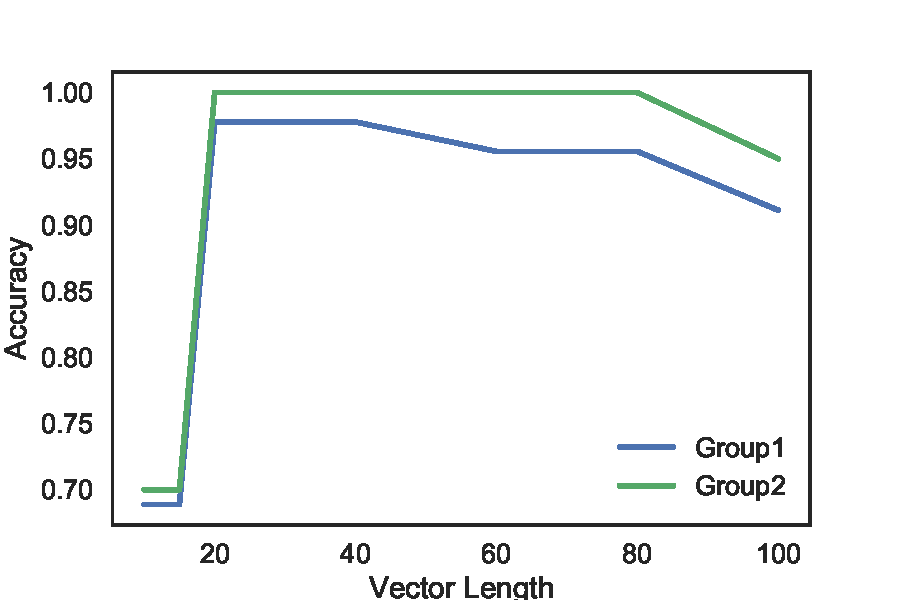
\includegraphics[width=\textwidth]{img/curve3.pdf}
        \caption{Fitting Observed Facts}
        \label{fig:sensitive-best-accuracy-1}
        %\vspace{-0.3em}
    \end{subfigure}
    \begin{subfigure}[]{0.23\textwidth}
        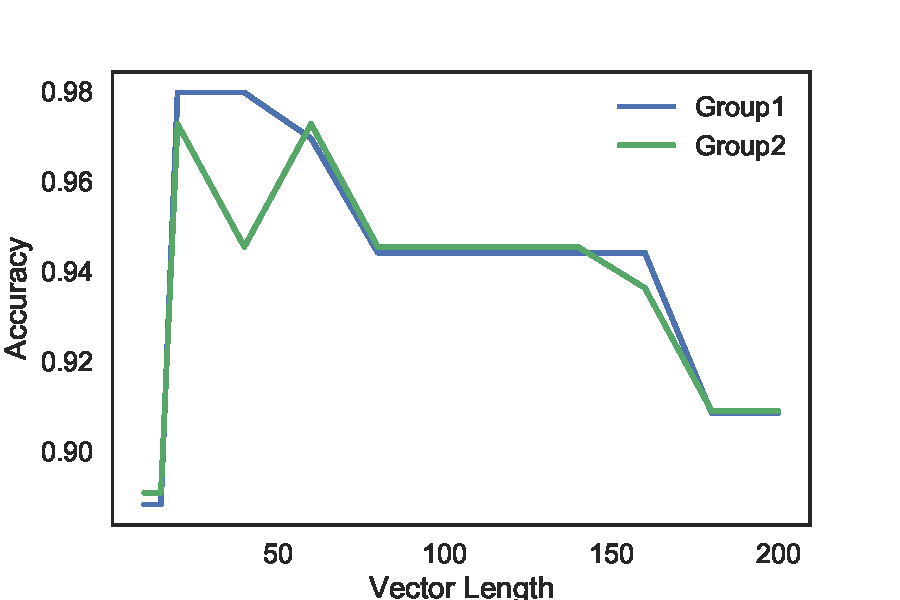
\includegraphics[width=\textwidth]{img/curve4.pdf}
        \caption{Learning from Rules }
        \label{fig:sensitive-best-accuracy-2}
        %\vspace{-0.3em}
    \end{subfigure}
    \caption{Best Accuracy w.r.t. Vector Length.}
    \label{fig:sensitive}
    % \vspace{-1.2em}
\end{figure}

\begin{table*}[t]
    \centering
    \begin{tabularx}{\textwidth}{L{0.2\textwidth}|L{0.35\textwidth}|L{0.35\textwidth}}
        \toprule
        Model X & Feature of Model X  & Feature of LTN \\
        \midrule
        Markov Logic \newline Network \cite{wang2008hybrid}
        &
        -The level of truth of a formula depends on the number of models that satisfy the formula

        -Works under the closed world assumption
        &
        -The level of truth of a complex formula is -determined by (fuzzy) logical reasoning

        -Works under open domain
        \\
        \midrule
        Bayesian Logic \cite{milch20071}
        &
        Explicit probabilistic approach
        &
        Take the benefits of tensor networks for computational efficiency.
        \\
        \midrule
        Knowledge \newline Embedding \cite{rocktaschel2015injecting}
        &
        -Function-free langauges

        -A special case of LTN

        -The semantics of the universal and existential quantifiers is based on the closed-world assumption (CWA)

        &
        -Provide groundings for functional symbols

        -A General model

        -Does not make the CWA

        -No specific t-norm
        \\
        \bottomrule
    \end{tabularx}
    \caption{Comparison with Similar Model}
    \label{tab:compare}
\end{table*}

In this part, we want to test the effect of vector length. We enumerate the vector length from 1 to 100 and shows the best accuracy on two groups. We did our experiments on both observed data and weighted dataset with rule. As the performance of C-LNT is better than LNT, we only shows the result of C-LNT, which is shown in Figure \ref{fig:sensitive}.

Figure \ref{fig:fitting-best-accuracy-1} shows the result in observed dataset.
From this figure, we can conclude that the performance is not always getting better with the increase of vector length. That's may because the under training problem. That is, as the

Actually, we want to find the appropriate vector lenght that is enough for fitting the data
